\chapter{Bayes}

\vspace{1em}
\hfill
\begin{minipage}[c]{0.55\textwidth}
\raggedleft
\small\itshape
The actual science of logic is conversant at present only with things either certain, impossible, or entirely doubtful, none of which (fortunately) we have to reason on. Therefore the true logic for this world is the calculus of probabilities.\\[0.5em]
\upshape\footnotesize James Clerk Maxwell, 1850
\end{minipage}%
\hspace{0.5em}
\begin{minipage}[c]{0.12\textwidth}
% \includegraphics[width=\textwidth]{figures/ch01_bayes.png}
\end{minipage}
\vspace{1.5em}

\noindent Suppose a friend tells you they flipped a coin five times and every flip came up heads.

What should you believe?

There are at least two hypotheses worth taking seriously. The coin might be ordinary and your friend got lucky. Five heads in a row on a fair coin happens once in every thirty-two trials, which is unusual but not rare. Alternatively, the coin might be a trick coin, weighted to always land heads. Such coins exist; some are sold as novelties.

Before your friend mentioned the experiment, you had some sense of how common trick coins are. Probably very low. Most coins are fair. Trick coins exist but are unusual.

After your friend's report, your belief should change. The data, five heads in a row, fits a trick coin more comfortably than a fair coin. Not impossibly for a fair coin. Just more comfortably for a trick one.

How much should your belief change?

This is the question Bayes' theorem answers. Given:

\begin{itemize}
\item Your prior belief about how common trick coins are.
\item The probability of five heads on a fair coin.
\item The probability of five heads on a trick coin (which is one, every time).
\end{itemize}

You can compute exactly the new probability that this coin is trick.

This chapter is about that calculation, where it comes from, and why it is the only consistent way to do it.

\section*{Belief as counting}

Strip away the formula for a moment.

Imagine a population of ten thousand coin-flipping trials. Before the data, you believe one percent of all such trials use a trick coin. So about one hundred trials use trick coins; about nine thousand nine hundred use fair coins.

Now restrict your attention to the trials that produced HHHHH.

Every trick-coin trial produced HHHHH (trick coins always do), so all hundred trick-coin trials are in the restricted set.

Fair-coin trials produced HHHHH only about one time in thirty-two. So about three hundred and nine of the nine thousand nine hundred fair-coin trials are in the restricted set.

The restricted set contains roughly $100 + 309 = 409$ trials. Of those, $100$ are trick-coin trials.

The fraction of trick-coin trials within the restricted set is

$$\frac{100}{409} \approx 0.24.$$

Your belief that this particular coin is trick, after seeing the data, should be about twenty-four percent.

That is the entire calculation. Counting, then counting again after restriction. Figure~\ref{fig:bayes-counting} shows the populations before and after.

\begin{figure}[h]
\centering
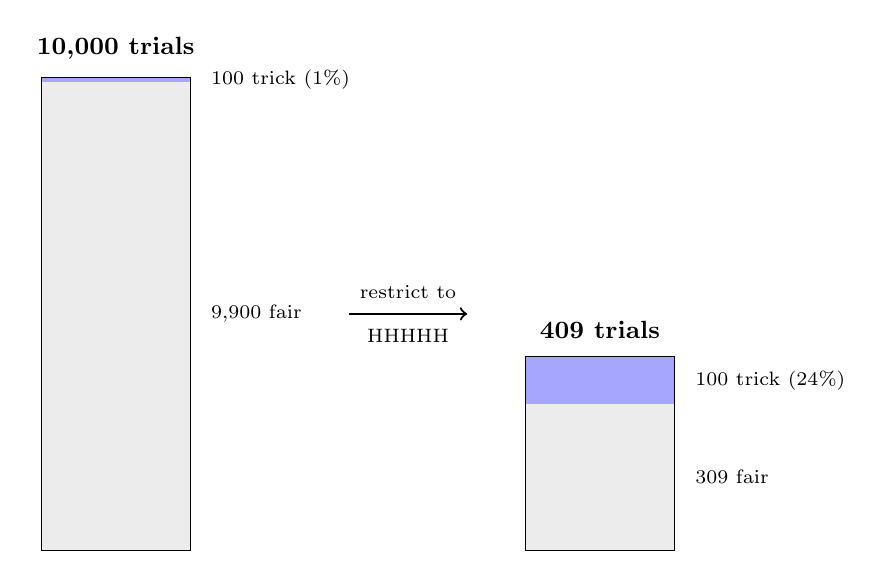
\begin{tikzpicture}[scale=0.75]
  % Left rectangle: prior population (10,000 trials), height 8 units
  \draw[thick] (0,0) rectangle (2.5,8);
  \fill[blue!35] (0,7.92) rectangle (2.5,8);
  \fill[gray!15] (0,0) rectangle (2.5,7.92);
  \node[anchor=south, font=\small\bfseries] at (1.25,8.15) {10{,}000 trials};
  \node[anchor=west, font=\scriptsize] at (2.7,7.96) {100 trick (1\%)};
  \node[anchor=west, font=\scriptsize] at (2.7,4) {9{,}900 fair};

  % Arrow
  \draw[->, thick] (5.2,4) -- (7.2,4);
  \node[anchor=south, font=\scriptsize] at (6.2,4.1) {restrict to};
  \node[anchor=north, font=\scriptsize] at (6.2,3.9) {HHHHH};

  % Right rectangle: restricted population (409 trials), height 3.27 units
  \draw[thick] (8.2,0) rectangle (10.7,3.27);
  \fill[blue!35] (8.2,2.47) rectangle (10.7,3.27);
  \fill[gray!15] (8.2,0) rectangle (10.7,2.47);
  \node[anchor=south, font=\small\bfseries] at (9.45,3.42) {409 trials};
  \node[anchor=west, font=\scriptsize] at (10.9,2.87) {100 trick (24\%)};
  \node[anchor=west, font=\scriptsize] at (10.9,1.24) {309 fair};
\end{tikzpicture}
\caption{The Bayesian update as counting. Left: the prior population of $10{,}000$ trials, $1\%$ trick coins (the thin blue band). Right: restricted to the $409$ trials that produced HHHHH. Every trick-coin trial survives (trick coins always produce HHHHH); only about $309$ of the $9{,}900$ fair-coin trials do. Within the restriction, the trick fraction has grown from $1\%$ to about $24\%$, not because any individual trial changed, but because the data restricted the count.}
\label{fig:bayes-counting}
\end{figure}

The data did not prove anything. The coin might still be fair and your friend might have gotten genuinely lucky. The data restricted the population of trials consistent with what you observed, and within that restricted population, the proportion of trick-coin trials changed.

This is what an update is: restriction to a subset, followed by counting within.

\section*{Bayes' theorem}

The formula is what you get when you write the counting argument with symbols.

Let $H$ stand for the hypothesis ``this is a trick coin'' and $D$ stand for the data ``five heads in a row.'' We want $P(H \mid D)$: the probability the coin is trick, given the data.

By the counting argument,

$$P(H \mid D) = \frac{\text{count of trick-coin trials that produced } D}{\text{count of all trials that produced } D}.$$

The numerator counts the trick-coin trials that produced the data. With symbols, that is the total count of trick-coin trials times the fraction of those that produced the data: $P(H) \cdot P(D \mid H)$.

The denominator counts all trials that produced the data, split by hypothesis:

$$P(D) = P(H) P(D \mid H) + P(\neg H) P(D \mid \neg H).$$

Putting them together,

$$P(H \mid D) = \frac{P(D \mid H) P(H)}{P(D)}.$$

This is Bayes' theorem. It looks more imposing than the counting. It is the counting, with names for the pieces. Figure~\ref{fig:bayes-restriction} shows the geometry.

\begin{figure}[h]
\centering
\begin{tikzpicture}[>=Stealth, scale=1.0]
  % Outer box
  \draw[thick] (0,0) rectangle (10,5);
  \node[anchor=north east, font=\small\itshape] at (9.85,4.85) {all coin trials};

  % Circle H (hypothesis)
  \draw[thick, blue] (3.8,2.5) circle (1.7);
  \fill[blue, fill opacity=0.15] (3.8,2.5) circle (1.7);
  \node[blue, anchor=south, font=\bfseries] at (2.5,3.7) {$H$};

  % Circle D (data)
  \draw[thick, red] (6.2,2.5) circle (1.7);
  \fill[red, fill opacity=0.15] (6.2,2.5) circle (1.7);
  \node[red, anchor=south, font=\bfseries] at (7.5,3.7) {$D$};

  % Label in intersection
  \node[font=\small] at (5.0,2.5) {$H \cap D$};
\end{tikzpicture}
\caption{Bayesian updating as restriction. The outer rectangle is the space of all possible coin trials. The blue circle $H$ contains the trials where the coin is trick. The red circle $D$ contains the trials that produced five heads. After the data, only trials in $D$ are still in play. The posterior $P(H \mid D) = |H \cap D| / |D|$ is the fraction of the restricted population that is also in $H$. Bayes' theorem is what you get when you write this fraction in terms of the original sizes.}
\label{fig:bayes-restriction}
\end{figure}

The named pieces:

\begin{itemize}
\item $P(H)$ is the \emph{prior}. What you believed before the data.
\item $P(D \mid H)$ is the \emph{likelihood}. How likely the data was, assuming the hypothesis.
\item $P(D)$ is the \emph{evidence}. How likely the data was at all, summed over hypotheses.
\item $P(H \mid D)$ is the \emph{posterior}. What you should believe after the data.
\end{itemize}

The formula moves you from prior to posterior. Given the prior and the likelihoods, the posterior is forced.

\section*{Why this is the only consistent way}

There are other rules you could imagine for combining beliefs and evidence. Many have been proposed. Almost none survive contact with simple consistency requirements.

Suppose your rule combines two independent pieces of evidence by adding their support. You see evidence supporting the hypothesis to degree $0.6$. You see a second independent piece, also supporting to degree $0.6$. Adding gives $1.2$. But a degree of belief is bounded by certainty; it cannot exceed $1$. The rule produces nonsense at the boundary, which means it is producing nonsense in proportion everywhere short of the boundary.

Or suppose your rule produces different conclusions depending on the order in which evidence arrives. You see $D_1$ then $D_2$ and conclude one thing. You see $D_2$ then $D_1$ and conclude another. The evidence is the same. A consistent agent reaches the same conclusion either way. The order in which two pages of a letter are read should not change what the letter says.

In 1946, the physicist R. T. Cox showed that the consistency requirements needed to avoid these and similar pathologies, taken together, force the calculus of belief revision to be probability theory. Strictly, force it to be isomorphic to probability theory, which is the same thing up to renaming.\footnote{Cox's original proof has had loose ends tightened by later authors. A counterexample by Halpern (1999) showed the argument requires an additional regularity condition on the domain; modern treatments (Jaynes, Paris, Van Horn) either assume this or restrict the setting. The qualitative conclusion is not in dispute.}

The requirements are modest:

\begin{itemize}
\item Degrees of belief are real numbers.
\item Two paths to the same conclusion give the same answer.
\item The calculus reduces to classical logic when certainty is reached.
\end{itemize}

The conclusion is sharp. Any agent whose belief revision is internally consistent, who reaches the same conclusion no matter the order of evidence, and who respects logic where logic suffices, is doing Bayesian updating.

Whether or not they call it that. Whether or not they have read this chapter. Whether or not they know it.

This is a load-bearing result for the rest of the book. Bayesian updating is not one option among many. It is the unique calculus of consistent belief. Any other rule, applied consistently, eventually contradicts itself.

\section*{What Bayes does not tell you}

The theorem is precise. Cox's result makes it unique. Together they specify how you should update beliefs in the presence of evidence.

They do not specify where you should start.

In the coin example, the prior was ``one percent of coins are trick.'' That number came from somewhere. Past experience with coins, presumably. But past experience with coins gives you a probability over coins by, presumably, Bayesian updating. Which requires a prior over coins. Which had to come from somewhere.

The regress goes all the way down.

A reasonable agent could start with $P(\text{trick}) = 0.5$, treating fair and trick coins as equally likely a priori. After five heads, they would land at about $0.97$.

Another reasonable agent could start with $P(\text{trick}) = 0.001$. After the same five heads, they would land at about $0.031$.

Both are using Bayes. Both are internally consistent. Both answer the same question with the same data. They land in different places because they started in different places. Cox's theorem does not adjudicate. Bayes' theorem does not either.

This is the problem of induction returning in a new form. Hume said there is no logical justification for inferring future from past. Bayes says: given a prior, here is how to do the inference. The hard part of Hume's problem, the part that resists, is the same one. Where does the prior come from?

\section*{Where this leaves you}

You now have a procedure for updating beliefs. The procedure is unique. Any consistent agent uses it, whether they have noticed or not.

You also have a hole. The procedure requires a prior the procedure itself does not supply. Different priors give different posteriors. The math does not pick between them.

The next chapter looks at the prior problem in more detail and shows why it is harder than it first appears. Chapter 3 introduces the bridge between description length and probability. Chapter 4 takes the bridge to its limit and arrives at the universal prior, the unique optimal prior in a sense Chapter 4 will make precise.

By the end of Part I, the hole in Bayes is closed. The closing comes with a price. The optimal prior is uncomputable. The rest of the book is about what that means for any agent, biological or mathematical or machine, that has to act in the world with bounded resources.
